\chapter{Implementation}

\section{Meta Model and Instantiation}
Our system has a simple meta model for describing (nested) classes and their methods. The graphical user interface operates exclusively on the meta model and makes changes to it. The meta model can then be instantiated to generate the actual classes. When changes to the meta model are made, these changes can also be applied to already existing instantiations of the model, allowing giving programmers the feeling of working with a live system.

\paragraph{Smalltalk-80 Class/Meta Model}
Squeak already comes with a meta model: objects are instances of a classes, consequently, classes are also instances of a class. In Smalltalk, every class is an instance of its own meta class, which is in turn instance of \texttt{Metaclass}.

Our system allows class generation at runtime: class generator methods generate classes along with their respective meta classes. Therefore, we need a specification/blueprint that describes how a class generator method should construct a class. At first glance, it might seem logical to use meta classes; after all, a meta class is the class of a regular (non-meta) class and classes are instance generators. However, meta classes cannot be used as class object generators in a way required by our system for two reasons.

Firstly, meta classes do not have any information about their non-meta class counterpart: for example, they do not know anything about their instance methods or their instance variables. Instantiating a meta class would not generate a functional class object, which is why Smalltalk prohibits generating new instances of a meta class. In fact, the class \texttt{ClassBuilder} is used to create new classes and it always creates class objects alongs with their meta class objects.

Secondly, our system supports defining methods on the instance side and on the class side. Consequently, we do not only need to generate class object but also meta class objects. All meta classes are an instance of \texttt{Metaclass}. But if we wanted to generate different meta classes, we would need a different \texttt{Metaclass} class, each of which generates its corresponding meta class. In some programming languages, the instance-of chain carries on infinitely; Ruby is an example. However, in Smalltalk, every meta class is an instance of \texttt{Metaclass} and this is where the instance-of chain recurses: \texttt{Metaclass} is an instance of \texttt{Metaclass class}, which is an instance of \texttt{Metaclass}.

For this reason, we cannot use the Smalltalk-80 meta model to generate new classes on the fly and use our own simple meta model instead.

\paragraph{Nested Classes Meta Model}
Figure~\ref{fig:impl_meta_model} shows the meta model in our system. The meta model is built around specifications: there are specifications for classes, meta classes, and methods. A specification describes how its corresponding object is built. \texttt{ClassSpecification}s generate classes, \texttt{MetaclassSpecification}s generate meta classes, and \texttt{MethodSpecification}s generate methods. Since classes cannot exist without their respective meta classes, a class specification is always linked with its meta class specification and vice-versa. When a class specification is instantiated, the system generates both the class and the meta class. Meta class specifications cannot be instantiated.

\begin{figure}
	\centering
	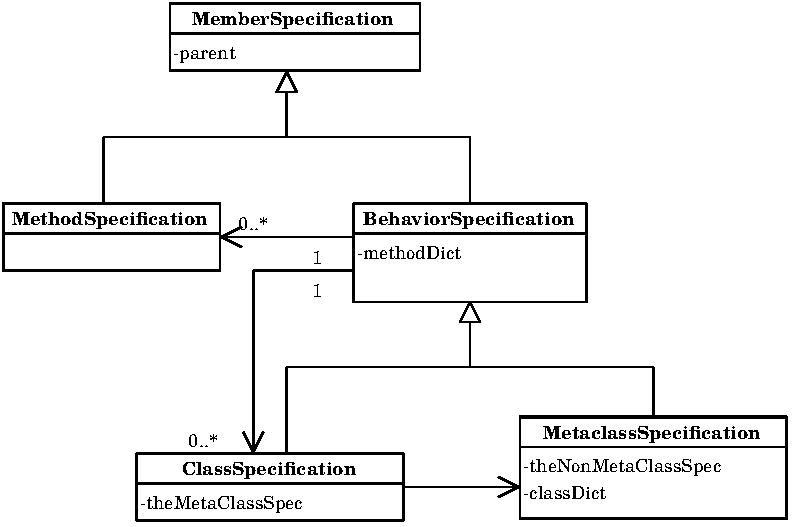
\includegraphics[scale=1]{metamodel.pdf}
	\caption{Meta Model for Nested Classes}
	\label{fig:impl_meta_model}
\end{figure}

\paragraph{Class Specifications}
A class specification describes classes. It has a collection of \texttt{MethodSpecification}s, representing instance methods of the class. Upon instantiation, all method specifications are instantiated within the target class. For every class specification, there is a corresponding method specification containing the source code of the class generator method in the parent's method dictionary. This method specification determines (when executed in the running system) to which class the methods will be added (\emph{target class}). Top-level classes are an exception: they are always a new subclass of the class \texttt{Module}.

\paragraph{Meta Class Specification}
A meta class specification describes meta classes. It has a collection of \texttt{MethodSpecification}s, representing class methods of the class (i.e., instance methods of the meta class). Upon instantiation, all method specifications are instantiated within the targer class' meta class. Consequently, meta classes do not method specifications associated with.

However, meta classes can have nested classes of their own. For every class defined in a meta class, there is a corresponding method specification present in the method dictionary (see previous paragraph).

\paragraph{Method Specification}
A method specification describes methods. It contains the source code of the method and stores information necessary for class caching and UI metadata. Whenever a method specification is instantiated, the method source code is compiled in the target class. 

Note, that different byte code must be generated for different target classes: for example, instance variable reads and write are compiled to parameterized\footnote{There are separate bytecodes for reading the first or second instance variable etc.} \texttt{pushRcvr:} and \texttt{popIntoRcvr:} bytecodes, where instance variables are referenced with their index\footnote{The first instance variable has index 0, second index variable has index 1, etc.}. In addition, the \texttt{outer} and the \texttt{enclosing} keyword must be bound to different method literals, depending on the lexical scope of the class.

\paragraph{Class Initialization}
Figure~\ref{fig:lazy_class_gen} illustrates how the system generates and initializes a nested class (class specification instantiation).

\begin{figure}
	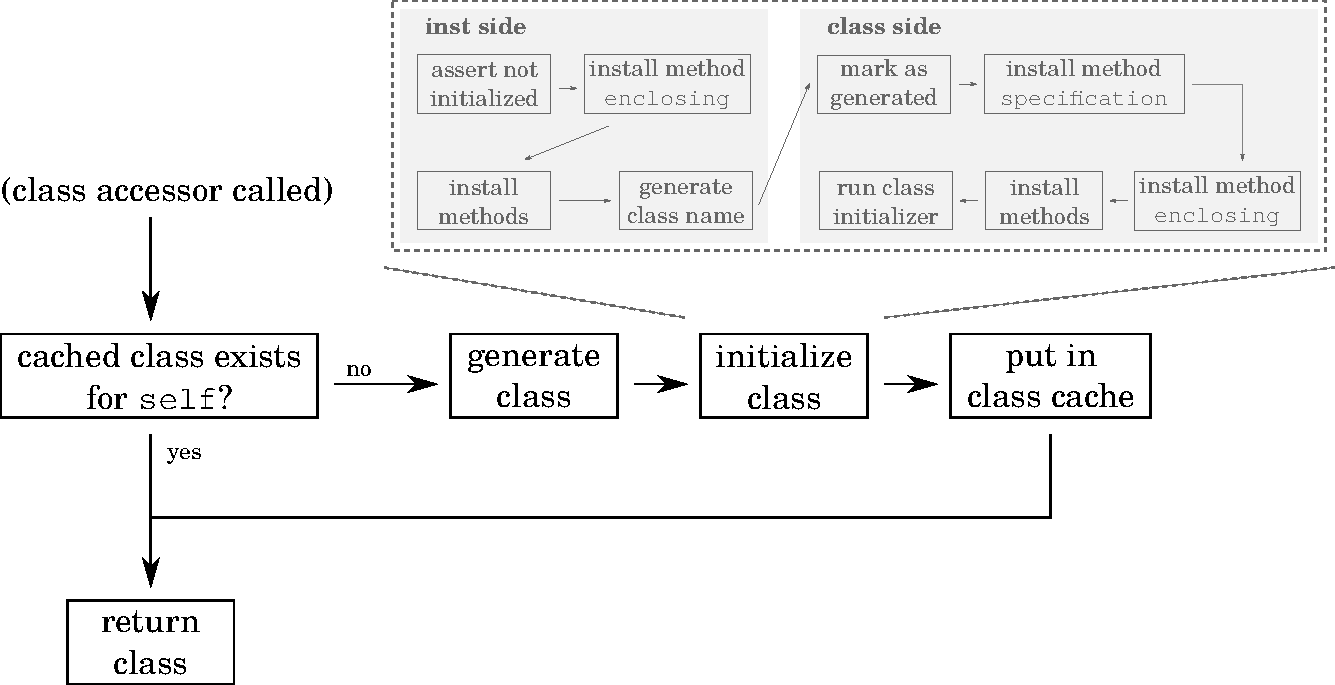
\includegraphics[width=\textwidth]{lazy_class_gen.pdf}
	\centering
	\caption{Lazy class generation and initialization}
	\label{fig:lazy_class_gen}
\end{figure}

Whenever a class accessor method is invoked, the method first checks if the class is already cached. If that is the case, it is returned. Otherwise, the class generator method called, returning an empty uninitialized class, i.e., all instance methods are still missing and only the superclass and the instance and class variables are set up correctly. The following list gives an overview of the steps necessary for initializing a class.

\begin{enumerate}
	\item Install \texttt{enclosing} instance method. This method returns the enclosing class.
	\item Install/compile all instance methods listed in the class specification.
	\item Generate the class name. The class name is a concatenation of the enclosing class' name and the selector of this class' accessor method. It is stored as an instance variable at \texttt{Class}. Note, that every class object is an instance of its meta class, which is a subclass of \texttt{Class}.
	\item Add a marker method to the meta class to mark it as generated. This makes is easy to check if a class is an ordinary (legacy) Smalltalk class or was generated within our system.
	\item Install \texttt{specification} class method. This method returns the class specification, which is useful for meta programming purposes.
	\item Install \texttt{enclosing} class method. This method is identical to the instance method.
	\item Install/compile all class methods listed in the meta class specification.
	\item Send \texttt{initialize} to the class object.
\end{enumerate}

Note, that class initialization is lazy. A class is only generated and initialized if the corresponding accessor method was called. All references to classes in the source code actually call the accessor method, making sure that the class is available when it is needed. 

Class generator methods can return subclasses of other classes; the superclass is referenced by calling the accessor method. Compared to the default package-loading process in Squeak, this makes class creation easier. In Squeak, the system has to analyze which classes are subclasses of each other, in order to create classes in the correct order (superclass has to exist before subclass is created). In our system, classes are created when their accessor method is called, and if these classes depend on another superclass, that superclass is created when the class generator method calls its accessor method (if it does not already exist).

\paragraph{Class Accessor Methods and Class Generator Methods}
For a nested class, two methods are installed on the meta class object: a class generator method, returning the class to which methods should be added (usually a newly-created subclass), and a class accessor method, checking whether the class was already created and is in the cache or calling the class generator method, otherwise.

The selector for the class accessor method is the name of the class. The selector for the class generator method is the same selector, but with a dollar sign prefix. This ensures that the method can only be called by using meta programming from our system, and also avoids accidential name clashes with other methods. For example, if a class is named \texttt{Foo}, the class accessor method has the selector \texttt{Foo} and the class generator method has the selector \texttt{\$Foo}.

\section{Anonymous Classes and Subclass Generation}
In Smalltalk, new classes are created by subclassing an already existing class. Squeak has special class, the \texttt{ClassBuilder}, containing all the functionality for creating the class object, the meta class object, giving the class a name, possibly migrating the old class and its instances (if an existing class was changed), and registering it in the \texttt{globals} dictionary.

Our system reuses the class builder and adds functionality for creating anonymous subclasses. Anonymous subclasses do not have a name and certain checks are omitted (e.g., if the class name starts with a capital letter). Also, anonymous subclasses are not added to the \texttt{globals} dictionary.

\paragraph{Subclass Notation}
Figure~\ref{fig:impl_subclass_squeak} shows how subclasses are created in Squeak. The first statement is a message send to \texttt{Object} which not only creates the subclass but also adds it to the \texttt{globals} dictionary. The second statement is also executable code that adds an instance variable to the meta class object. The difference between class variables and class instance variables is that class variables are shared among all subclasses, whereas class instance variables have different values for every class object~\cite{classvar1,classvar2}. For example, if \texttt{A} has a class variable \texttt{Bar} and \texttt{B} is a subclass of \texttt{A}, then both \texttt{A} and \texttt{B} share one variable \texttt{Bar}.

\begin{figure}[!htp]
\begin{lstlisting}
Object subclass: #NewClass
    instanceVariableNames: 'foo bar'
    classVariableNames: 'Bar'
    poolDictionaries: ''
    category: 'Demo-Experiments'.

NewClass class
	instanceVariableNames: 'Foo'.
\end{lstlisting}
\caption{Subclass notation in Squeak}
\label{fig:impl_subclass_squeak}
\end{figure}

Figure~\ref{fig:impl_subclass_nested} shows how subclassesa created in our system. \texttt{NewClass} is a class generator method and also the name of the new class. Therefore, it is no longer necessary to pass a symbol with the name of the new class to the \texttt{subclass:} method. Note, that the \textttt{<class>} pragma is necessary to distinguish between class generator methods and regular methods, which might accidentially return a class. Only in the former case, a class specification object is created.

\begin{figure}[!htp]
\begin{lstlisting}
NewClass
    < class >
    ^ Object 
    	subclassWithInstVars: 'foo bar'
    	classVars: 'Bar'
        classInstVars: 'Foo'
\end{lstlisting}
\caption{Subclass notation with nested classes}
\label{fig:impl_subclass_nested}
\end{figure}


\section{\texttt{thisOuter} and \texttt{thisScope}}

\section{Class Updates}
using instances weak array on specification

\section{Integration in Squeak}

\subsection{Module Repository}
replacement for Smalltalk dict

\subsection{IDE Support}
works in workspace, test runner. How to write tests? New system browser

\subsection{Debugger}
shows slightly different code (thisContext automatically inserted, generator methods)